% Official MNRAS class, unmodified. Scientific prose converted from reviewed Markdown.
\PassOptionsToPackage{hyperfootnotes=false}{hyperref}
\PassOptionsToPackage{sort&compress}{natbib}
\RequirePackage{fix-cm}
\pdfminorversion=5
\documentclass[fleqn,usenatbib]{mnras}
% Use superscripted numeric citations and a numbered reference list while
% retaining the MNRAS document class and bibliography formatting.
\setcitestyle{numbers,super,open={},close={},citesep={,}}
\renewcommand{\bibnumfmt}[1]{[#1]}
\usepackage{newtxtext,newtxmath}
\usepackage[T1]{fontenc}
\usepackage{graphicx,amsmath,booktabs,longtable}
\usepackage{xurl}
\usepackage{microtype,balance}
\raggedbottom
% Avoid duplicate anchors with the class caption definition and current hyperref.
\makeatletter
\patchcmd{\caption}{\refstepcounter}{\H@refstepcounter}{}{\PackageError{bhns}{Caption compatibility patch failed}{Check hyperref compatibility.}}
% The official BST purifies undated labels to nd[a-d]; display readable n.d. citations.
\apptocmd{\NAT@parse}{%
\ifdefstring{\NAT@date}{nda}{\def\NAT@date{n.d.a}}{}%
\ifdefstring{\NAT@date}{ndb}{\def\NAT@date{n.d.b}}{}%
\ifdefstring{\NAT@date}{ndc}{\def\NAT@date{n.d.c}}{}%
\ifdefstring{\NAT@date}{ndd}{\def\NAT@date{n.d.d}}{}%
}{}{\PackageError{bhns}{Undated citation patch failed}{Check natbib compatibility.}}
\makeatother
\DeclareRobustCommand{\VAN}[3]{#2}
\let\VANthebibliography\thebibliography
\def\thebibliography{\DeclareRobustCommand{\VAN}[3]{##3}\VANthebibliography}
\newcommand{\AuthorTODO}[1]{\textbf{TODO: #1}}
\hypersetup{hidelinks,pdftitle={black hole and neutron star Classification Beyond Known Sources},pdfauthor={Author information pending}}

\title[BH/NS classification beyond known sources]{Black Hole and Neutron Star Classification Beyond Known Sources: An RXTE/PCA Evaluation}
\author[Youhan Wanigasuriya]{Youhan Wanigasuriya$^{1}$\thanks{youhanwanigasuriya@gmail.com}\\
$^{1}$University of Colombo}
\date{Submission and acceptance dates to be supplied by the publisher}
\pubyear{2026}
\begin{document}
\label{firstpage}
\pagerange{\pageref{firstpage}--\pageref{lastpage}}
\maketitle

\begin{abstract}

Machine-learning discrimination between black-hole (BH) and neutron-star (NS) X-ray binaries is often evaluated using repeated observations of a limited number of physical systems. When observations of the same binary occur in both training and testing, strong performance need not imply generalization to an unseen system. We investigate this distinction using a provenance-controlled reconstruction of 687 RXTE/PCA observations from 7 BH and 22 NS systems, comparing observation-wise and source-disjoint evaluation with conventional logistic-regression and random-forest classifiers. Under source-grouped evaluation, logistic regression achieves a source-level AUROC of 0.948 (95\% conditional source-bootstrap interval 0.844--1.000), with balanced accuracy of 0.786, showing that useful BH/NS ranking remains after complete physical-source exclusion. A source-label randomization control provides a complementary result: after the true BH/NS mapping is destroyed while each source retains one randomized label, median random-forest AUROC remains 0.942 under observation-wise evaluation but falls to 0.461 under source-grouped evaluation. This demonstrates exploitable source-associated structure under repeated-source overlap without identifying its physical origin. Source-disjoint ranking also persists after independently executed HEASoft/CALDB processing, under common instrumental-support restrictions, and in an expanded independently processed cohort containing 9 BH and 22 NS systems. Fixed-threshold classification is less stable than ranking. Physical spectral-state independence remains unresolved: the pre-specified state-matched analysis was not performed because the common hard-dominated regime contained 6 BH but only 4 NS systems, below the required five per class. These results show that BH/NS spectral ranking can transfer across held-out systems in the selected RXTE/PCA cohort, while also demonstrating why physical-source separation is required when performance is interpreted as transfer to previously unseen astronomical systems.

\end{abstract}
\begin{keywords}
\end{keywords}

\section{Introduction}
\label{sec:1}

Identifying the compact object in an X-ray binary is important for studies of accretion physics and the Galactic population of stellar remnants. Secure black hole (BH) and neutron star (NS) classifications, however, require evidence that is not uniformly available across observed systems. Dynamical measurements provide strong support for BH classifications \citep{CorralSantana2016}, whereas thermonuclear X-ray bursts and coherent pulsations provide direct evidence for NS systems \citep{Galloway2020,Sanna2018}. Catalogues assembled from such evidence are therefore an important basis for supervised classification. In particular, class labels should not be assigned solely from the spectral appearance that a classifier is subsequently asked to predict \citep{CorralSantana2016,Galloway2020}.

X-ray spectra nevertheless contain substantial information about the emitting accretion flow. Their observed form is not determined by compact-object class alone: accretion state, source history, absorption, observing conditions and instrumental response can all contribute to the measured representation \citep{Belloni2005,Gladstone2007,Jahoda2006}. RXTE studies of neutron star state transitions also illustrate why a single hardness coordinate cannot automatically be interpreted as a universal physical state variable across systems \citep{Gladstone2007}. Consequently, a classifier may successfully separate BH and NS observations without having isolated a unique physical signature of the central object.

Machine learning methods have previously demonstrated substantial discriminatory power for X-ray binaries. \citet{Gopalan2015} applied a probabilistic Gaussian process approach to RXTE All Sky Monitor colour--colour--intensity coordinates \citep{Vrtilek2013}, including predictions for known systems withheld from training. \citet{Pattnaik2021} used RXTE/PCA spectra with random-forest classifiers and explicitly examined observation-wise, source-wise and leave one source out evaluation. \citet{deBeurs2022} similarly evaluated complete-source exclusion with MAXI/GSC colour--colour--intensity data and addressed unequal source representation through source-aware subsampling. More recent work has combined spectral and phenomenological information in neuro-parametric classification \citep{Garg2026}. These studies establish both the promise of X-ray-binary classification and important precedents for evaluating generalization across physical systems.

A central difficulty, however, is that the statistical unit represented by an X-ray spectrum is not necessarily the scientific unit over which generalization is desired. A dataset may contain hundreds or thousands of observations while representing only a comparatively small number of independent binaries. Repeated observations increase the number of measured spectra, but they do not create an equivalent number of independent physical systems. This distinction matters whenever the intended use of a classifier is to make predictions for a previously unseen binary rather than for an additional observation of a source already represented during training.

Observation-wise and source-disjoint evaluation therefore answer different questions. In an observation-wise split, observations of the same physical system may occur in both training and test sets. Such an evaluation asks whether another observation can be classified when the model may already have encountered the same underlying system. In a source-disjoint split, all observations belonging to a held-out physical system remain outside training, so the evaluation instead tests transfer across systems. Both settings can be scientifically meaningful, but performance in the former does not by itself establish performance in the latter. Correlated or source-associated structure may support prediction when the same physical systems occur on both sides of the split \citep{Pattnaik2021,Wright2015,Neto2019}.

The unresolved question is therefore not whether whole-source validation is possible or whether it has been used previously. Rather, it is how much apparent BH/NS discrimination can be supported by repeated-source structure itself, how much discrimination remains when complete physical systems are withheld, and how robust that conclusion is to alternative instrumental processing and sample restrictions. This distinction is particularly important for astronomical applications in which a classifier may ultimately be asked to assist with systems not represented in its training catalogue.

We address this problem using a source-level randomization control in addition to conventional source-disjoint testing. The astrophysical class labels are permuted among physical sources while preserving the number of sources in each class, and every observation belonging to a given source retains the same randomized label. This destroys the association between the true BH/NS class and the source while preserving the repeated-source organization of the data. If these arbitrary source-level labels remain predictable under observation-wise splitting, the result demonstrates that repeated-source overlap can provide exploitable predictive structure even in the absence of the true astrophysical class mapping. Source-grouped evaluation provides the corresponding test after that access route is removed. The control is intended to diagnose source-associated structure; it does not by itself identify whether that structure is astrophysical, instrumental, observational or a combination of these effects \citep{Neto2019}.

The present study therefore asks three linked questions. First, how much BH/NS discrimination survives when complete physical systems are withheld from model training? Second, can observation-wise evaluation predict arbitrary labels attached to physical sources after the genuine astrophysical mapping has been destroyed? Third, do conclusions from source-disjoint evaluation persist under independently executed RXTE/PCA processing and detector-support restrictions? We additionally investigate whether the available literature provides a sufficiently diverse set of BH and NS systems in a justified common spectral regime for a confirmatory state-controlled comparison.

To answer these questions, we construct a provenance-controlled RXTE/PCA dataset with independently reviewed source identities and physical labels, evaluate conventional logistic-regression and random-forest classifiers under observation-wise, source-grouped and leave-one-source-out designs, apply source-level label-randomization controls, repeat the analysis with an independently executed HEASoft/CALDB reduction, and examine detector-support and metadata sensitivities. We also retain an explicit feasibility criterion for the proposed state-controlled comparison rather than relaxing it after inspection of the available systems. Source-disjoint evaluation itself is established practice \citep{Gopalan2015,Pattnaik2021,deBeurs2022}; the contribution of the present study is the combination of physical-source isolation, source-randomization diagnostics, provenance-controlled reconstruction, instrumental validation and explicit limits on the astrophysical interpretation of the resulting classifier performance.

\section{Study design and analysis framework}
\label{sec:2}

The analysis is organized around the physical source as the principal unit of inference. Observation-wise evaluation permits different observations of the same binary to occur in training and testing, whereas source-disjoint evaluation withholds complete physical systems. The two designs are compared using the same primary observations, so that the principal difference is the evaluation unit rather than the underlying dataset. Headline performance is summarized after aggregating predictions within each physical source. We deliberately use conventional classifiers because the focus of the study is the evaluation design and its interpretation rather than optimization of model architecture.

Figure~\ref{fig:1} summarizes the analysis framework. The primary branch compares observation-wise, source-grouped and leave-one-source-out evaluation. A source-label randomization control tests whether repeated-source overlap can support prediction after the true BH/NS association has been removed. An instrumental-validation branch repeats source-disjoint evaluation after independently executed HEASoft/CALDB processing, compares the original and independently processed representations on identical admitted ObsIDs, and applies restrictions designed to improve comparability of detector support. A subsequently expanded independently processed cohort evaluates the same source-disjoint framework with additional admissible physical systems. A separate state-control branch tests whether the literature-supported catalogue contains the pre-specified minimum number of independent BH and NS systems in a justified common spectral regime; the confirmatory state-matched experiment is performed only if that feasibility criterion is satisfied.

Analysis protocols were frozen locally at successive project stages before execution of the corresponding tests, with retained hashes and versioned inputs. These stage-frozen protocols are not presented as an externally registered preregistration. Later sensitivity analyses are identified separately from the corresponding frozen analyses. Manuscript generation reads completed outputs and does not alter model selection rules or the stage-frozen feasibility criterion.

\begin{figure*}
\centering
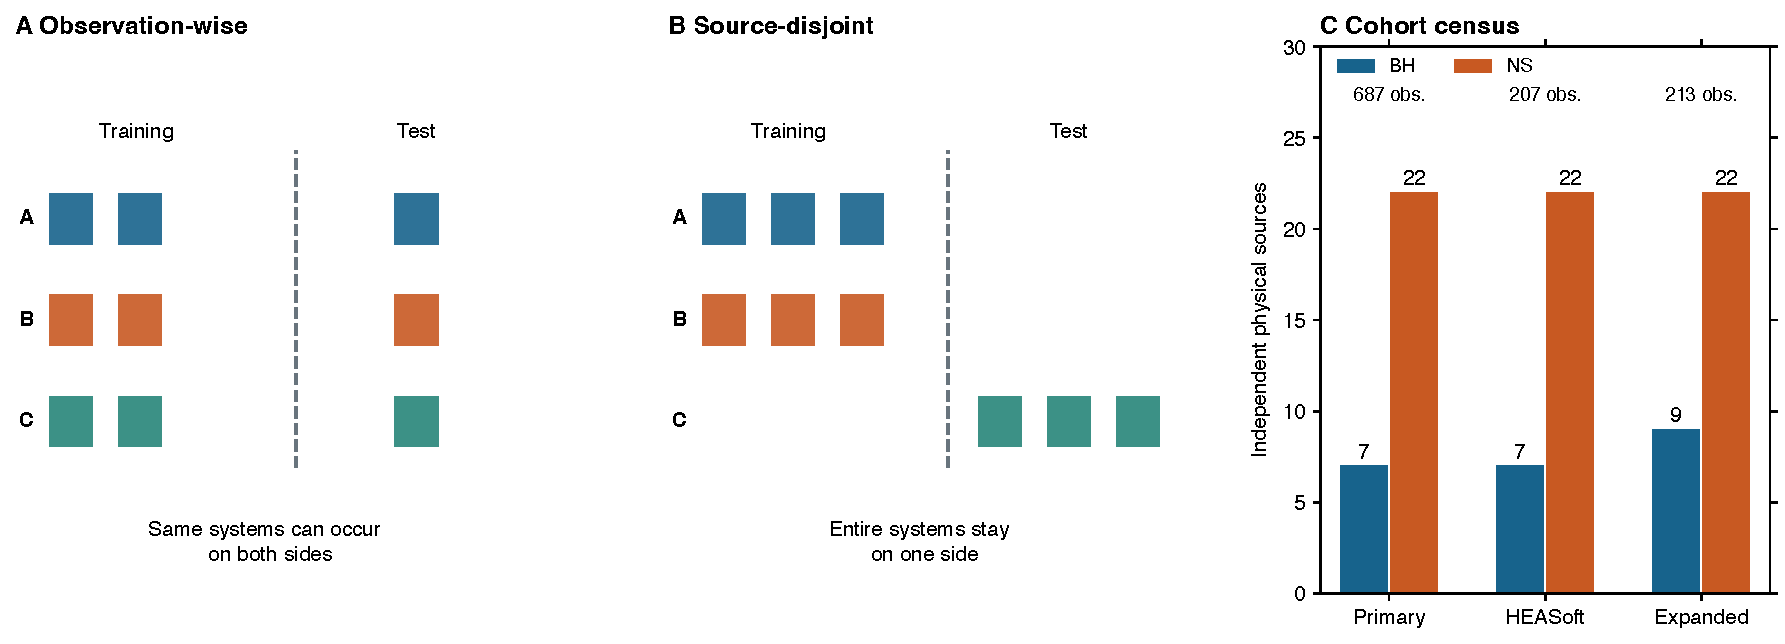
\includegraphics[width=\textwidth]{figures/figure_1_design.pdf}
\caption{Analysis design. (A) Observation-wise evaluation permits different observations of the same physical system in training and test sets. (B) Source-disjoint evaluation withholds complete systems. (C) Numbers of independent BH and NS systems in the primary, independently processed and expanded cohorts. The HEASoft branch represents independent processing rather than an independent draw of the source population. Schematic cells are illustrative and do not denote actual fold membership.}
\label{fig:1}
\par\smallskip
\begin{minipage}{\textwidth}
\footnotesize
\textbf{Alt text:} A split-design schematic contrasts repeated observations shared between training and testing with whole-source exclusion; a separate panel shows the numbers of independent BH and NS systems across processing cohorts.
\end{minipage}
\end{figure*}

\section{RXTE/PCA dataset reconstruction}
\label{sec:dataset}

\subsection{Source census and class labels}

The starting roster comprised 61 entries and reported 14\,885 observations. Following independent identity review, 30 canonical target identities were retained for archive querying. BH inclusion used a conservative, dynamically supported subset of BlackCAT, whereas NS inclusion required published thermonuclear-burst or coherent-pulsation evidence, using MINBAR and primary alias references \citep{CorralSantana2016,Galloway2020}. Spectral appearance was not used to assign or resolve the physical class label, and uncertain candidates were excluded.

Aliases were mapped to canonical physical-source identifiers before any data split was constructed. V4641~Sgr and SAX~J1819.3$-$2525, for example, were treated as a single physical system \citep{Orosz2001}. An inherited BH classification for IGR~J17379$-$3747 was not retained because published pulsation evidence supports an NS identification \citep{Sanna2018}; this source ultimately contributed no accepted primary observation. Ambiguous attributions arising from crowded fields or discrepant catalogue names were excluded rather than resolved using model predictions. The complete source evidence, alias mapping and exclusion trail are provided in Supplement~S1.

\subsection{Observation acquisition}

Archive queries returned 11\,996 distinct candidate ObsIDs, of which 9\,215 satisfied the reviewed name- and position-matching criteria. The maximum accepted pointing displacement was $0.05^\circ$. To limit domination by heavily observed systems while retaining temporal coverage, at most 32 observations per source were selected at approximately evenly spaced chronological ranks, including the temporal endpoints. This deterministic sampling rule does not constitute random sampling of either the available observations or the underlying X-ray-binary population.

The selection procedure yielded 858 observations. Of these, 841 had complete spectral-product sets and 808 could be reconstructed successfully. After application of the observation-quality and source-sufficiency criteria, 687 observations remained in the primary cohort. Acquisition failures, missing products and subsequent exclusions were recorded separately. Observations with incomplete products were excluded rather than imputed.

\subsection{Spectral reconstruction}

The analysis uses data from the Rossi X-ray Timing Explorer (RXTE) Proportional Counter Array (PCA). The primary reconstruction used mission-generated Office of Guest Investigator Programs (OGIP) Standard2 source, modelled-background and response products \citep{NASAStandard}. FITS identity, instrument designation, ObsID history, channel ordering, exposure, detector selection, good-time intervals (GTIs), formal statistical errors and response-energy bounds were checked before an observation was retained. PCA calibration is described by \citet{Jahoda2006}. These mission-generated products were not independently re-reduced for the primary branch, and no additional manual deadtime correction was applied at this stage.

Let $D$ and $B$ denote the source and background count vectors, respectively; $t$ their exposures; $a$ their AREASCAL factors; and $b$ their BACKSCAL factors. The net detector rate follows the OGIP scaling convention \citep{XSPECSpectra}:

\begin{equation}
\label{eq:net-rate}
R =
\frac{D}{t_D a_D}
-
\frac{b_D}{b_B}
\frac{B}{t_B a_B}.
\end{equation}

For the primary summed-detector products, the resulting rate and its statistical error were divided by the number of selected proportional counter units (PCUs). Source and background variances were propagated using the squared scaling factors. This convention is specific to the primary summed-PCU products and was not assumed for the independently processed HEASoft branch.

All retained spectra were mapped to a common detector-space representation containing 43 equal-width intervals between 5 and 25~keV. For native interval $j$ and output interval $i$, $W_{ij}$ is the fractional overlap of the native interval with the output interval. The rebinned rate vector is

\begin{equation}
\label{eq:overlap}
R_{\mathrm{out}} = W R ,
\end{equation}

where the transformation assumes constant rate density within each native interval. The corresponding covariance matrix is propagated as

\begin{equation}
\label{eq:covariance}
\operatorname{Cov}(R_{\mathrm{out}})
=
W\,\operatorname{Cov}(R)\,W^{\mathsf{T}} .
\end{equation}

Integrated-band variances therefore use the full propagated covariance rather than only its diagonal. Signed net-rate bins were retained. The resulting features are correlated detector-space count rates, not statistically independent channels or unfolded photon fluxes.

\subsection{Quality control, provenance and exclusions}

An observation was retained only when the source, background, error and response arrays were finite and valid, source identity was verified, exposure was positive, and the integrated net rate over the analysis band exceeded 5~counts~s$^{-1}$ per selected PCU. The primary reconstruction additionally required at least four usable observations per physical source. The later independently processed HEASoft cohort used a minimum of two observations per source; these thresholds belong to distinct, frozen analysis branches. Formal statistical errors do not include calibration or background-model systematic uncertainties.

The reconstruction records the input paths, download status, transformations and retained hashes for each product. Source-sufficiency criteria were applied only after observation-level quality filtering. Physical class labels and ambiguous source identities were not inferred from spectral shape. The resulting dataset is therefore a provenance-controlled reconstruction based on the reviewed source roster and public archive products rather than an exact replication of an unavailable private input selection.

\subsection{Primary and validation cohorts}

The primary cohort contains 687 observations from 29 independent physical systems: 122 observations from 7 BH systems and 565 observations from 22 NS systems. The independently processed HEASoft validation cohort contains 207 observations from the same physical-source roster. Restricting the primary and independently processed representations to their defined common instrumental support retains 598 and 201 observations, respectively.

The expanded independently processed cohort contains 213 observations from 31 physical systems: 9 BHs and 22 NSs. GRO~J1655$-$40 and GRS~1915+105 provide the two additional BH systems, whereas V404~Cyg supplied no usable observation under the frozen quality criteria. The number of independent systems is therefore substantially smaller than the number of individual spectra, and the BH/NS source counts remain unequal.

Because the primary, independently processed, common-support and expanded cohorts differ in observation selection and/or processing, each reported performance estimate is identified by its corresponding cohort.

\section{Machine learning methodology}
\label{sec:4}

\subsection{Features and models}

The primary predictors are the reconstructed detector-space count rates described in Section~\ref{sec:dataset}. Source identifier, ObsID, target name and physical class label are excluded from the input matrix. Recorded statistical errors, normalized spectral shape and detector metadata are considered only in separately identified sensitivity analyses and do not enter the primary feature definition. Standardization changes the numerical scale of the predictors but does not remove instrument-response dependence or place different systems on a common physical luminosity scale.

NS is treated as the positive class. A fixed probability of 0.5 provides the reference prediction. Two conventional classifiers are used so that the analysis emphasizes evaluation design rather than model complexity. Logistic regression uses the \texttt{liblinear} solver, a maximum of 3000 iterations and inverse regularization strength

\[
C \in \{0.01,\,0.1,\,1,\,10\}.
\]

The random forest contains 100 trees, uses a minimum leaf size of 3, and considers maximum depths of 4 and unrestricted depth. Both models are implemented in scikit-learn \citep{Pedregosa2011}. No architecture search, post hoc ensemble or model family selection is performed.

\subsection{Source weighting}

Repeated observations from the same binary are not treated as equivalent to independent physical systems during model fitting. Within each training partition, observation $i$ from source $s$ receives a weight proportional to the reciprocal of the number of training observations available for that source,

\[
w_i \propto \frac{1}{n_s},
\]

with weights normalized to have mean unity within the training partition. Each physical source therefore contributes equal total training weight irrespective of how many retained observations it provides.

This weighting limits domination by heavily observed systems but does not make repeated observations statistically independent. It also does not equalize total BH and NS class weight because the numbers of independent systems in the two classes differ.

\subsection{Evaluation designs}

Three evaluation designs are used to distinguish prediction of additional observations from generalization to unseen physical systems.

Observation-wise evaluation uses five stratified outer folds and generates out-of-fold predictions for every retained observation. Different observations of the same physical source may occur in both training and test partitions. This overlap is intentional: the experiment represents prediction of additional observations when the underlying system may already be represented during training, and it is not interpreted as unseen-source validation. Model selection within each outer training partition nevertheless uses a source-disjoint inner validation split.

For source-grouped evaluation, the canonical physical-source roster is stratified by class into five outer folds. All observations belonging to a test source are excluded from the corresponding outer training partition. Predictions from the held-out folds are subsequently combined and aggregated at the physical-source level. The same canonical source identity is used consistently for splitting, source weighting, prediction aggregation and uncertainty estimation.

Leave-one-source-out (LOSO) evaluation withholds one complete physical system at a time and trains on all remaining systems. The same feature definition, preprocessing and hyperparameter-selection rules used for the grouped analysis are retained. LOSO and five-fold grouped evaluation have different training-set sizes and compositions; differences between their reported scores therefore should not be interpreted as controlled comparisons between different algorithms or as evidence that one splitting scheme is intrinsically superior.

\subsection{Nested model selection and leakage prevention}

All preprocessing and hyperparameter selection are confined to the corresponding outer training partition. Each outer training set supplies a single 20\% stratified physical-source holdout for inner validation. Candidate hyperparameters are selected by source-level balanced accuracy; ties are resolved by choosing the first candidate in the frozen hyperparameter grid.

For each candidate model, \texttt{StandardScaler} is fitted only on the inner-training observations and then applied to the corresponding validation observations. After hyperparameter selection, the scaler and model are refitted using the complete outer training partition before prediction of the outer test data. No outer test source contributes to hyperparameter selection or scaler fitting in grouped or LOSO evaluation.

The primary pipeline performs no imputation, learned feature selection or principal-component transformation. Because the number of independent systems, particularly BH systems, is limited, inner source-level validation provides a relatively coarse criterion for model selection; the hyperparameter search is therefore intentionally restricted to the frozen small grids described above. Source-level prediction summaries are provided in Supplement~S3, and the repository retains the primary split definitions. The full fit-audit records, including selected hyperparameters and preprocessing provenance, are not included in this release. The principal random seed is 42.

\subsection{Source aggregation, metrics and uncertainty}

Headline performance is evaluated at the level of the physical source. Observation-level probabilities are clipped to $[10^{-7},\,1-10^{-7}]$ before transformation to log odds. For source $s$ with $n_s$ retained predictions, the aggregate source score is

\begin{equation}
\label{eq:source-score}
p_s =
\sigma\left[
\frac{1}{n_s}
\sum_{i=1}^{n_s}
\operatorname{logit}(p_{si})
\right],
\end{equation}

where $\sigma$ is the logistic function and $p_{si}$ is the predicted NS probability for observation $i$ of source $s$. The clipping prevents divergent log odds at probabilities of exactly zero or one. Averaging log odds provides one reproducible summary score per physical system and does not multiply repeated observations as though they were statistically independent.

For fixed-threshold classification, a source is assigned to the NS class when $p_s \geq 0.5$; ties are also assigned to NS. This fixed threshold is reported separately from ranking performance and is not optimized on the outer test predictions.

The primary performance metric is source-level area under the receiver operating characteristic curve (AUROC), which measures ranking across BH and NS systems without requiring a classification threshold. Balanced accuracy (BA), Matthews correlation coefficient (MCC), NS F1 score, average precision (AP) and Brier score provide complementary descriptions of fixed-threshold classification, precision--recall behaviour and probability quality. The field labelled \texttt{PR\_AUC} in the frozen analysis outputs corresponds to average precision. These source-level quantities should not be interpreted as ordinary observation-level accuracy.

Uncertainty intervals are 95\% percentile intervals from 2000 class-stratified bootstrap resamples of physical sources, conditional on the completed out-of-fold predictions. For paired comparisons, identical physical sources are resampled together. The bootstrap therefore reflects variation under source-level resampling of the fitted predictions, but it does not repeat preprocessing, hyperparameter selection or model fitting. It also does not represent uncertainty over a population-complete census of X-ray binaries. The reported intervals consequently have a narrower interpretation than full repeated-training or population-sampling uncertainty, and their resolution is limited by the small number of independent systems, particularly BHs.

\section{Primary evaluation results}
\label{sec:5}

\subsection{Performance across evaluation designs}

The principal question is whether BH/NS discrimination persists when complete physical systems are withheld from model training. Table~\ref{tab:performance} summarizes source-level performance under the three primary evaluation designs, with full secondary metrics reported in Supplement~S2.

Under source-grouped evaluation, logistic regression achieves an AUROC of 0.948 [0.844, 1.000], with balanced accuracy (BA) of 0.786 and Matthews correlation coefficient (MCC) of 0.709. The random forest gives an AUROC of 0.909 [0.753, 1.000] and BA of 0.714. Source-level discrimination therefore remains strong after complete-source exclusion within the selected RXTE/PCA cohort. The uncertainty is determined by the limited number of independent physical systems, particularly BHs, rather than by the much larger number of individual spectra.

Observation-wise evaluation gives higher point estimates: AUROC is 0.987 for logistic regression and 0.994 for the random forest, with BA of 0.857 for both models. These scores are aggregated at the physical-source level from out-of-fold observation predictions, but observations of the tested systems may also occur in the corresponding outer training partitions. They therefore quantify performance in a repeated-source setting and are not interpreted as unseen-source validation.

Leave-one-source-out (LOSO) evaluation provides a complementary whole-source test. Logistic regression reaches an AUROC of 0.994 [0.961, 1.000] with BA of 0.714, whereas the random forest reaches 0.948 [0.844, 1.000] with BA of 0.786. The very high logistic LOSO AUROC does not translate into equally high fixed-threshold classification performance. More generally, AUROC measures ordering of source scores, whereas BA depends on the fixed decision threshold. Differences between LOSO and five-fold grouped estimates should not be interpreted as performance gains from one splitting scheme because their training-set compositions and sizes differ.

Figure~\ref{fig:2} shows the distinction between source-level ranking and fixed-threshold classification across the three evaluation designs.

\subsection{Observation-wise versus source-disjoint performance}

To quantify the change associated with repeated-source overlap, we compare observation-wise and source-grouped AUROC using paired source-level resampling. The observation-minus-grouped AUROC difference is 0.039 [0.000, 0.117] for logistic regression and 0.084 [0.000, 0.227] for the random forest.

Both conditional intervals include zero. The point estimates are higher under observation-wise evaluation, but this paired comparison alone does not establish a precisely measured nonzero inflation in AUROC for the true BH/NS labels. The source-label randomization experiment in Section~\ref{sec:6} therefore provides a complementary and more direct test of whether repeated-source overlap exposes exploitable source-associated structure.

\begin{table*}
\centering
\caption{Primary source-level performance across evaluation designs. Brackets give 95\% conditional source-bootstrap intervals for AUROC; BA uses the fixed 0.5 threshold. Full secondary metrics and numerical precision are reported in Supplement~S2. The three rows use the same primary cohort and should not be interpreted as independent replications.}
\label{tab:performance}
\small
\setlength{\tabcolsep}{5pt}
\begin{tabular}{lccccc}
\toprule
Evaluation design &
Obs. / sources &
Logistic AUROC [95\% interval] &
BA &
Forest AUROC [95\% interval] &
BA \\
\midrule

Observation-wise &
687 / 29 &
0.987 [0.942, 1.000] &
0.857 &
0.994 [0.961, 1.000] &
0.857 \\

Source-grouped &
687 / 29 &
0.948 [0.844, 1.000] &
0.786 &
0.909 [0.753, 1.000] &
0.714 \\

LOSO &
687 / 29 &
0.994 [0.961, 1.000] &
0.714 &
0.948 [0.844, 1.000] &
0.786 \\

\bottomrule
\end{tabular}
\end{table*}

\begin{figure*}
\centering
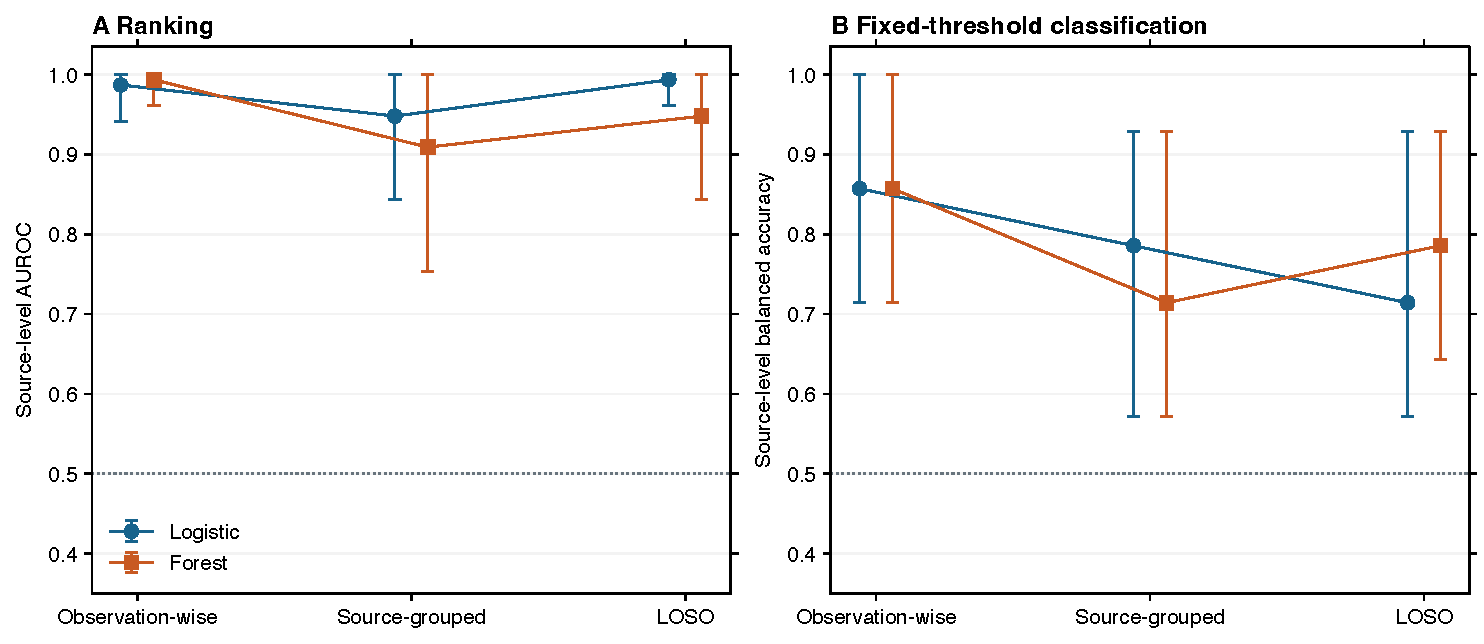
\includegraphics[width=\textwidth]{figures/figure_2_primary.pdf}
\caption{Primary source-level AUROC and balanced accuracy for observation-wise, source-grouped and leave-one-source-out evaluation. Error bars show conditional source-bootstrap intervals and do not include repeated fitting, hyperparameter-selection or fold-assignment uncertainty. The horizontal reference denotes chance ranking or balanced accuracy. The fixed 0.5 reference predictor is reported in Supplement~S2.}
\label{fig:2}
\par\smallskip
\begin{minipage}{\textwidth}
\footnotesize
\textbf{Alt text:} Two panels compare source-level AUROC and balanced accuracy across observation-wise, source-grouped and leave-one-source-out evaluation, with separate markers for logistic regression and random forest and conditional source-bootstrap interval bars.
\end{minipage}
\end{figure*}

\section{Controls for source-associated structure}
\label{sec:6}

\subsection{Source-label randomization}

The comparison between observation-wise and source-grouped performance on the true BH/NS labels cannot by itself determine whether repeated-source overlap exposes predictive information associated with physical-source identity. We therefore performed a source-level label-randomization diagnostic that destroys the true astrophysical class mapping while preserving the repeated-source structure of the dataset.

Class labels were permuted among physical sources while preserving the numbers of BH and NS labels. Every observation belonging to a given source retained the same randomized label. Observation-wise and source-grouped folds were then regenerated with stratification on the randomized labels. The diagnostic used a fixed unrestricted-depth random forest with the otherwise frozen forest settings and no hyperparameter tuning. Each randomized experiment therefore asks whether an arbitrary label attached to a physical source can be predicted when repeated observations of that source are either permitted or excluded across the training--test boundary.

Across 50 permutations of the primary cohort, the median source-level AUROC was 0.942 under observation-wise evaluation and 0.461 under source-grouped evaluation. Individual permutation outcomes are shown in Fig.~\ref{fig:3}. The large observation-wise values occur despite removal of the true BH/NS mapping, indicating that repeated-source overlap exposes predictive source-associated structure. By contrast, the grouped median is close to chance ranking, consistent with substantial removal of that access route when complete physical systems are withheld.

The same qualitative contrast is present in the independently processed HEASoft cohort. Across 10 permutations, the median AUROC is 0.769 under observation-wise evaluation and 0.503 under source-grouped evaluation. Because these are finite diagnostic ensembles rather than an exhaustive permutation distribution, they are not used as a formal significance test for the real-label classifiers.

The experiment establishes predictability associated with repeated physical sources, but it does not identify the origin of that information. Possible contributors include intrinsic source properties, accretion-state occupancy, observing history, instrumental response and other source-correlated measurement characteristics. We therefore use the term ``source fingerprint'' only as a descriptive shorthand for this predictability; the control does not establish literal memorization or a unique physical or instrumental mechanism.

\subsection{Source-identification diagnostic}

As a complementary exploratory test, we asked whether individual physical sources could themselves be distinguished from their observations. A multiclass random forest with 100 trees and minimum leaf size 2 was evaluated using three observation-level folds stratified by physical source. Preprocessing was fitted using training data only.

Mean per-source identification accuracy was 0.407, compared with approximately $1/29 = 0.034$ for uniform guessing among the 29 admitted source identities. This result provides additional evidence that the detector-space observations contain information associated with physical source identity. It is not, however, an additional estimate of BH/NS generalization and does not determine which astrophysical or instrumental properties support source identification.

Taken together, the randomization and source-identification diagnostics show that repeated observations contain exploitable source-associated structure. The stronger randomization result is the relevant control for interpreting the observation-wise BH/NS experiment: high performance when related observations occur in training and testing does not, by itself, establish transfer to a previously unseen physical system.

\begin{figure*}
\centering
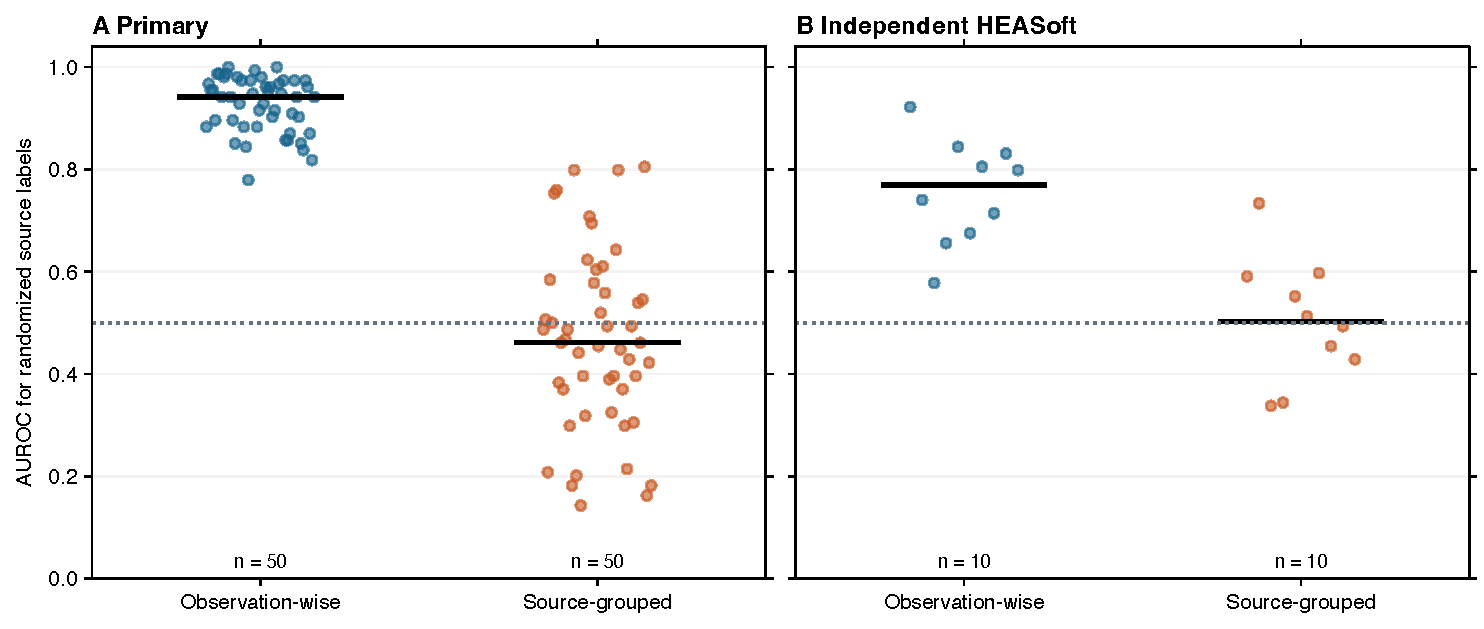
\includegraphics[width=\textwidth]{figures/figure_3_randomization.pdf}
\caption{Source-level AUROC for the frozen source-label randomization diagnostics in the primary and independently processed HEASoft cohorts. Each physical source retains one randomized label across all of its observations, while observation-wise and source-grouped evaluation differ in whether observations of the same physical system can occur on both sides of the training--test split. Points show individual permutations and median values are marked. Horizontal offsets are deterministic and used only for visibility. The horizontal reference denotes chance ranking. The displayed permutation distributions are diagnostic results and are not confidence intervals for the real-label classifiers.}
\label{fig:3}
\par\smallskip
\begin{minipage}{\textwidth}
\footnotesize
\textbf{Alt text:} Two panels show source-level AUROC values from randomized source labels under observation-wise and source-grouped evaluation in the primary and independently processed HEASoft cohorts. Observation-wise values are generally much higher than grouped values, and median markers are shown relative to a chance-ranking line.
\end{minipage}
\end{figure*}

\section{Instrumental robustness and cohort validation}
\label{sec:7}

\subsection{Independent HEASoft/CALDB processing}

To test whether the source-disjoint result depends strongly on the primary RXTE/PCA reconstruction, a separate processing branch was executed with HEASoft 6.37.1 \citep{HEASoft2014} and PCA Calibration Database (CALDB) release 20230501. The executed environment also records XSPEC 13.0.1, although no XSPEC-derived phenomenological fit parameters enter the classifiers.

Preselected ObsIDs from the original source roster were processed independently of the primary spectral products. At most eight chronological ranks per source were selected before validation performance was examined. The reduction used \texttt{pcaprepobsid}, \texttt{maketime} and \texttt{pcaextspect2}, with PCU2's top xenon layer, CALDB background estimation and a corresponding response \citep{NASAPCAext}. Good-time intervals required ELV $>10^\circ$, OFFSET $<0.02^\circ$, PCU2 active and ELECTRON2 $<0.1$. For the early-epoch reduction, time since South Atlantic Anomaly passage was additionally required to exceed 30~min or to carry the documented negative sentinel value \citep{NASAScreening}.

The independent reduction also differs from the primary products in deadtime and exposure handling. The live exposure already accounts for the contributing detector exposure and is therefore not divided by PCU count a second time \citep{NASAPCAext}. Rates and covariance are subsequently mapped to the same common detector-space representation used in the primary analysis. Because detector/layer selection, screening, background estimation, response construction and exposure handling change together, this branch tests robustness to the combined processing workflow rather than isolating the causal effect of any individual correction.

On the independently processed cohort, source-grouped AUROC is 0.903 for logistic regression and 0.896 for the random forest. Corresponding LOSO values are 0.922 and 0.896. Source-disjoint ranking therefore remains present after independently executed RXTE/PCA processing. This is a processing-robustness result and should not be interpreted as validation on an independently sampled astronomical population.

\subsection{Matched-observation and common-support comparisons}

Differences between the primary and HEASoft cohorts can arise both from processing and from which observations survive the respective workflows. We therefore performed a matched-observation comparison in which the original representation was refitted using exactly the ObsIDs admitted by the HEASoft reduction. On these identical observations, grouped and LOSO logistic-regression AUROCs are 0.909 and 0.916, respectively; corresponding random-forest values are 0.890 and 0.903.

For grouped evaluation, the paired HEASoft-minus-original AUROC difference is $-0.006$ [$-0.039$, 0.000] for logistic regression and 0.006 [0.000, 0.039] for the random forest. For LOSO evaluation, the corresponding differences are 0.006 [0.000, 0.039] and $-0.006$ [$-0.039$, 0.000]. All conditional intervals include zero (Supplement~S4). The matched comparison therefore provides no evidence for a large change in source-level ranking attributable to the alternative processing workflow within these observations. It does not establish equivalence of the two representations or eliminate the possibility of instrumental effects.

A complementary analysis restricts both representations to overlapping instrumental support. Strata combine PCA gain epoch and selected-PCU configuration, with at least two distinct physical systems from each class required in every retained stratum. Additional frozen restrictions require exposures between 256 and 16\,384~s, net rates between 5 and 1000~counts~s$^{-1}$ per PCU, background fraction no greater than 0.5, and at least two retained observations per source. These restrictions define overlapping support; they do not produce exact matching of the class-conditional instrumental distributions.

Within the restricted primary representation, grouped AUROC is 0.968 for logistic regression and 0.935 for the random forest. The corresponding values for the independently processed representation are 0.877 and 0.864. Thus source-level ranking remains present after restriction to the declared common instrumental support, although differences between these unequal subsets should not be interpreted as controlled processing effects. Figure~\ref{fig:4} summarizes both the matched-observation and common-support comparisons.

\subsection{Instrumental confounder diagnostics}

To assess whether recorded observational and detector metadata alone can reproduce the spectral classification result, we fitted models using observation year, log exposure, detector selection, native-channel coverage and gain-epoch indicators. Count-rate amplitudes, background fraction, source identity and response identifiers were excluded.

Under source-grouped evaluation, the metadata-only logistic model gives an AUROC of 0.701 [0.435, 0.922], whereas the random forest gives 0.604 [0.357, 0.825]. Balanced accuracy is 0.500 for both models. The recorded metadata therefore do not by themselves reproduce the source-level ranking obtained from the spectral representation in this design. This control does not exclude unrecorded confounding or interactions between instrumental conditions and spectral information.

Additional gain-epoch holdout and spectral-shape/background sensitivity analyses are reported in Supplement~S4. The feasible gain-epoch holdout contains too few independent systems for precise inference and is therefore treated as a sensitivity diagnostic rather than an additional validation result.

\subsection{Expanded physical-source cohort}

The independently processed branch was also extended beyond the original physical-source roster where usable observations satisfied the frozen quality criteria. The expanded cohort contains 213 observations from 31 physical systems: 9 BHs and 22 NSs.

Under source-grouped evaluation, logistic regression gives an AUROC of 0.919 and the random forest 0.889. Under LOSO evaluation, the corresponding values are 0.929 and 0.874. The expanded cohort therefore retains source-disjoint ranking after increasing the number of represented BH systems from seven to nine.

Figure~\ref{fig:5} displays the held-out LOSO score for every system in this expanded cohort. The figure also exposes the distinction between ranking and fixed-threshold classification: sources can be well ordered across classes while individual scores still fall on the wrong side of the fixed decision threshold. The expansion increases physical-source coverage but remains a small, selected RXTE/PCA cohort and is not prospective validation on a new survey or instrument.

\begin{table*}
\centering
\caption{Source-level performance in the independently processed, common-support and expanded validation cohorts. Brackets give 95\% conditional source-bootstrap intervals for AUROC; BA uses the fixed 0.5 threshold. Cohorts share physical systems and, in some comparisons, observations, and therefore should not be interpreted as independent replications.}
\label{tab:validation}
\small
\setlength{\tabcolsep}{4pt}
\begin{tabular}{llrrrr}
\toprule
Cohort / split &
Obs. / sources &
Logistic AUROC [95\% interval] &
BA &
Forest AUROC [95\% interval] &
BA \\
\midrule

HEASoft / grouped &
207 / 29 &
0.903 [0.753, 1.000] &
0.763 &
0.896 [0.760, 0.987] &
0.786 \\

HEASoft / LOSO &
207 / 29 &
0.922 [0.786, 1.000] &
0.763 &
0.896 [0.753, 0.987] &
0.714 \\

HEASoft common support / grouped &
201 / 29 &
0.877 [0.714, 0.981] &
0.763 &
0.864 [0.714, 0.974] &
0.763 \\

HEASoft common support / LOSO &
201 / 29 &
0.903 [0.766, 1.000] &
0.763 &
0.883 [0.740, 0.981] &
0.786 \\

Expanded / grouped &
213 / 31 &
0.919 [0.783, 1.000] &
0.889 &
0.889 [0.757, 0.980] &
0.722 \\

Expanded / LOSO &
213 / 31 &
0.929 [0.798, 1.000] &
0.811 &
0.874 [0.727, 0.970] &
0.699 \\

\bottomrule
\end{tabular}
\end{table*}

\begin{figure*}
\centering
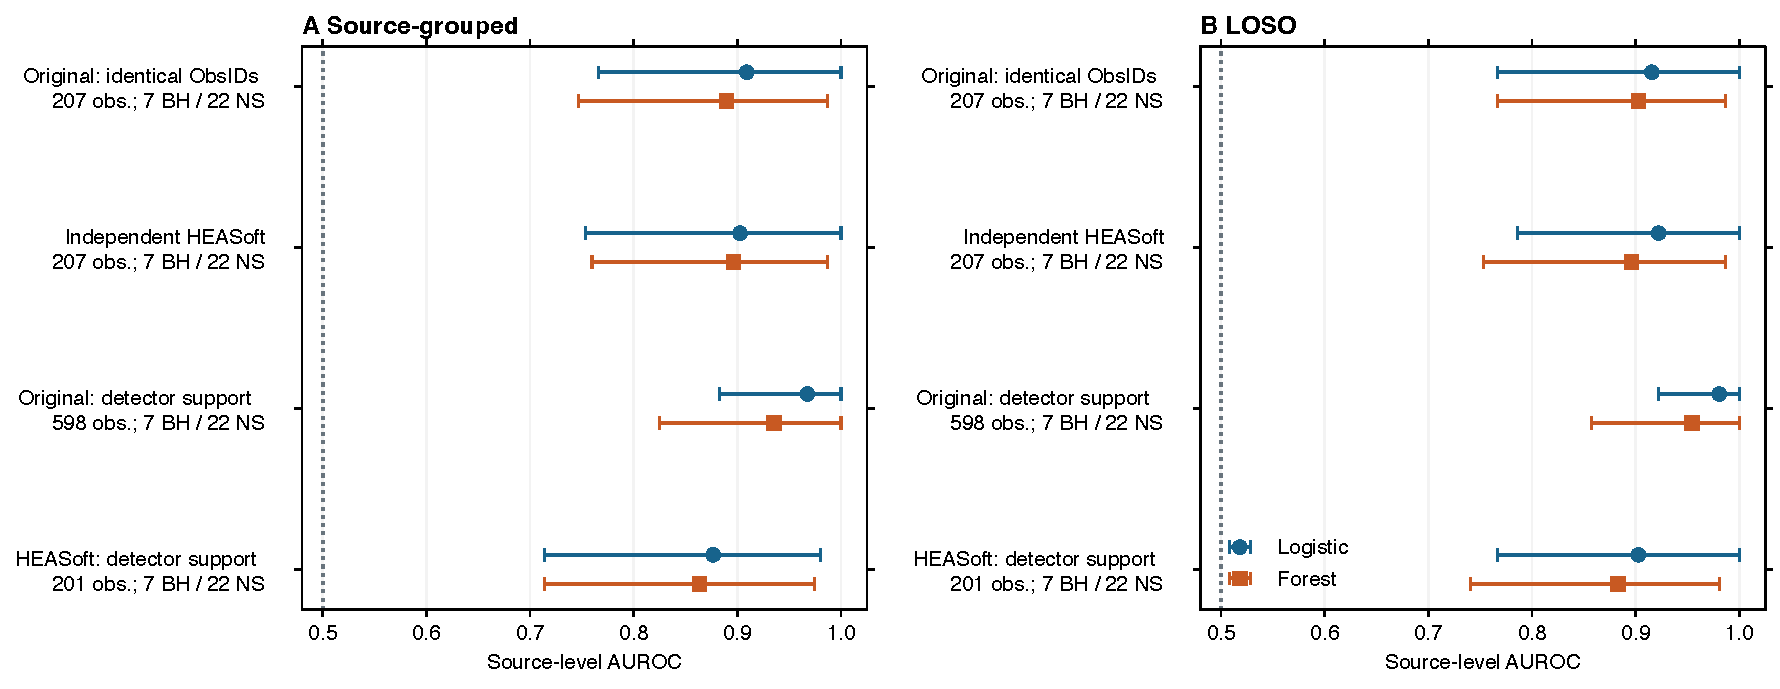
\includegraphics[width=\textwidth]{figures/figure_4_validation.pdf}
\caption{Source-level AUROC under matched-observation and common instrumental-support comparisons, shown separately for source-grouped and LOSO evaluation. The matched-observation comparison uses identical ObsIDs to distinguish processing differences from observation selection as far as the design permits. Common-support rows restrict the representations to the declared instrumental-support criteria but do not constitute exact distributional matching. Error bars are conditional source-bootstrap intervals.}
\label{fig:4}
\par\smallskip
\begin{minipage}{\textwidth}
\footnotesize
\textbf{Alt text:} Source-grouped and leave-one-source-out panels compare source-level AUROC for the original and independently processed representations on identical observations and after restriction to common instrumental support. Logistic-regression and random-forest results are shown with conditional source-bootstrap interval bars.
\end{minipage}
\end{figure*}

\begin{figure*}
\centering
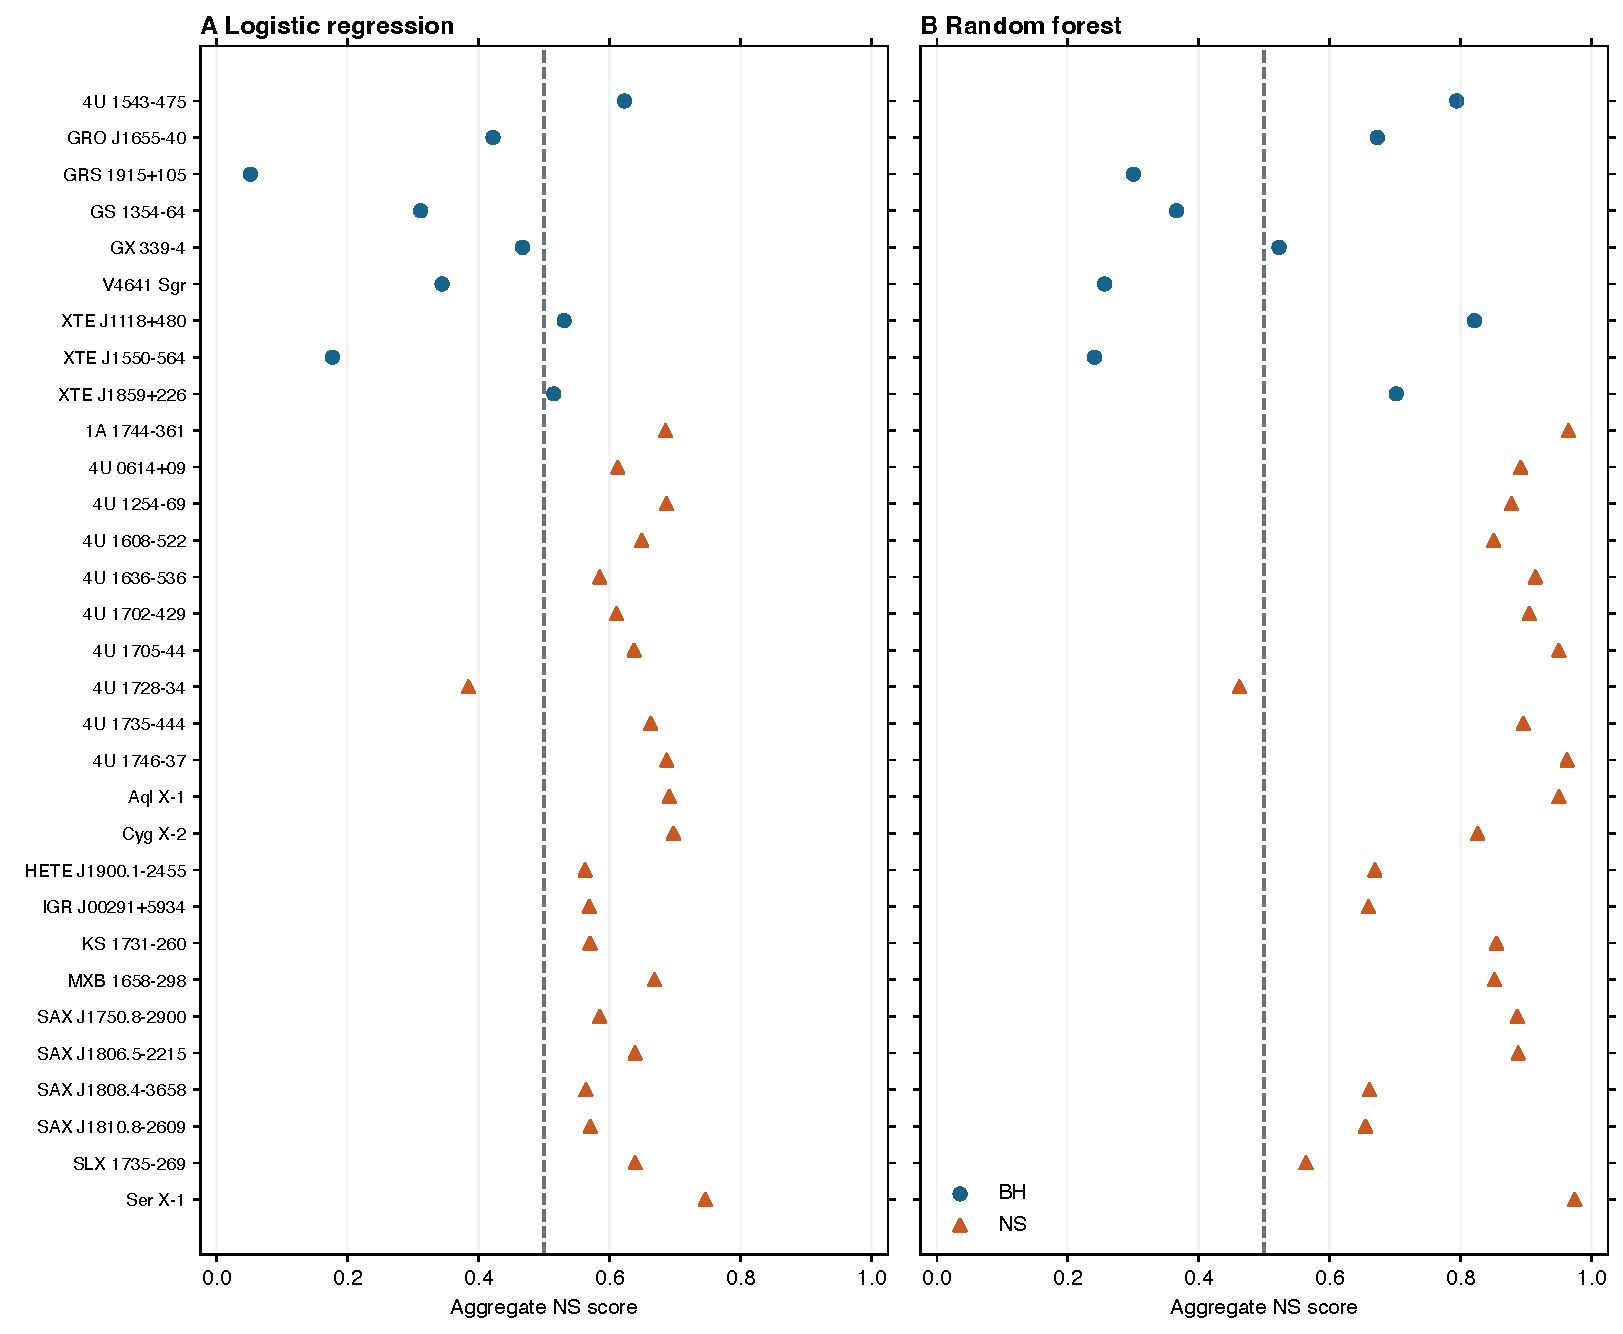
\includegraphics[width=\textwidth]{figures/figure_5_expanded.pdf}
\caption{Expanded-cohort LOSO aggregate NS scores for every physical system, shown separately for logistic regression and the random forest. BH and NS systems are distinguished by marker and colour, and the vertical line denotes the fixed classification threshold. Score ordering determines AUROC, whereas a source's position relative to the threshold determines its fixed-threshold classification. Aggregate scores are source-level summaries rather than calibrated posterior probabilities and do not have source-specific confidence intervals.}
\label{fig:5}
\par\smallskip
\begin{minipage}{\textwidth}
\footnotesize
\textbf{Alt text:} Two aligned panels show LOSO aggregate neutron-star scores for every physical system in the expanded cohort, separately for logistic regression and random forest. BH and NS systems use different markers, and a vertical line marks the fixed classification threshold.
\end{minipage}
\end{figure*}

\section{Spectral-state controls and feasibility}
\label{sec:9}

\subsection{State evidence and common-regime mapping}

Physical spectral-state dependence is a potential limitation of the source-disjoint BH/NS classification results. We therefore assembled an observation-level state catalogue from the literature and distinguished evidence according to its strength and applicability to individual RXTE observations. DIRECT assignments are tied to a specific ObsID, whereas STRONG assignments support the full observation interval. PROVISIONAL, unresolved and conflicting assignments are retained for provenance but are not used in the confirmatory state-matched analysis. Only justified DIRECT or STRONG evidence without unresolved ambiguity is considered eligible for that comparison.

Native BH and NS state labels are retained separately from any subsequent mapping to a shared hard- or soft-dominated regime. This distinction is necessary because the state taxonomies used for BH and NS systems are not universally interchangeable \citep{Belloni2005,Hasinger1989,Gladstone2007}. For example, an atoll island-state designation is not automatically treated as equivalent to a BH hard state; source-specific spectral evidence is required before an observation can be mapped to a common cross-class regime \citep{Gladstone2007}. Similarly, overlap between an ObsID and a published state interval is not considered sufficient when the complete observation is not supported. The full evidence hierarchy, mapping rules and observation-level assignments are provided in Supplement~S5.

A bounded literature extension was subsequently performed for 20 NS systems to identify additional observations with sufficiently specific state evidence. The extension added seven DIRECT native-state assignments. Of these, four observations from two physical systems satisfied the requirements for inclusion in a common hard-dominated regime: IGR~J00291+5934 \citep{Linares2007,Falanga2005} and the relevant SAX~J1808.4$-$3658 outburst \citep{Bult2015,Ibragimov2009}. A native-state assignment alone did not automatically qualify an observation for cross-class matching.

The extension was bounded to the declared literature search and processed observation set. Failure to identify additional qualifying observations therefore establishes feasibility only within those search bounds; it does not demonstrate that no useful state evidence exists elsewhere in the literature.

\subsection{Coarse hardness--intensity diagnostic}

As a separate diagnostic, we tested whether a much lower-dimensional detector-space representation preserves the class-associated ranking found with the full reconstructed spectrum. The frozen proxy representation uses

\begin{equation}
\log_{10}\left(\frac{\mathrm{mid}}{\mathrm{soft}}\right),
\qquad
\log_{10}\left(\frac{\mathrm{high}}{\mathrm{mid}}\right),
\qquad
\log_{10}\left(\mathrm{soft}+\mathrm{mid}+\mathrm{high}\right),
\end{equation}

with band boundaries corresponding to the fixed spectral representation at approximately 5.00, 9.65, 14.77 and 25.00~keV. Nonpositive or nonfinite band totals are excluded without clipping or imputation; all observations in the expanded cohort satisfy these requirements.

These coordinates describe detector-space hardness and intensity. They are not physical state labels, bolometric measurements or Eddington-normalized luminosities.

For logistic regression, the proxy representation gives a grouped AUROC of 0.965, compared with 0.919 for the full spectrum. Under LOSO evaluation, the corresponding values are 0.859 and 0.929. Paired proxy-minus-full AUROC intervals include zero in every comparison (Fig.~\ref{fig:6}; Supplement~S5).

Coarse hardness--intensity information therefore carries substantial BH/NS-associated ranking information in this cohort. The comparison does not demonstrate that the proxy and full-spectrum representations are equivalent, nor does it establish that spectral state completely mediates the classifier performance. In particular, a detector-space hardness coordinate is not a substitute for an independently justified physical state assignment.

\subsection{State-matched feasibility assessment}

The confirmatory state-controlled analysis was subject to a pre-specified, stage-frozen feasibility criterion requiring at least five independent physical systems from each class within a justified common regime. This criterion was retained unchanged after inspection of the available state evidence.

Following the literature extension, the hard-dominated regime contains six BH systems and four NS systems. The soft-dominated regime contains two BH systems and one NS system. Neither regime therefore satisfies the required minimum of five systems per class.

The confirmatory state-matched classifier was consequently not performed, and no state-controlled performance estimate exists. The shortfall should not be interpreted as a negative classification result: the planned experiment was not statistically admitted under its frozen feasibility rule.

Physical spectral-state independence is therefore not established by the present analysis. The strong source-disjoint ranking may reflect intrinsic compact-object information, differences in state occupancy, coarse hardness/intensity structure, other source-associated properties, or a combination of these effects. The proxy diagnostic shows that coarse spectral coordinates already contain substantial class-associated information, but it does not identify their physical origin. Relaxing the source-diversity requirement after observing the available state counts would change the confirmatory question, so the original criterion and the resulting limitation are retained.

\begin{figure*}
\centering
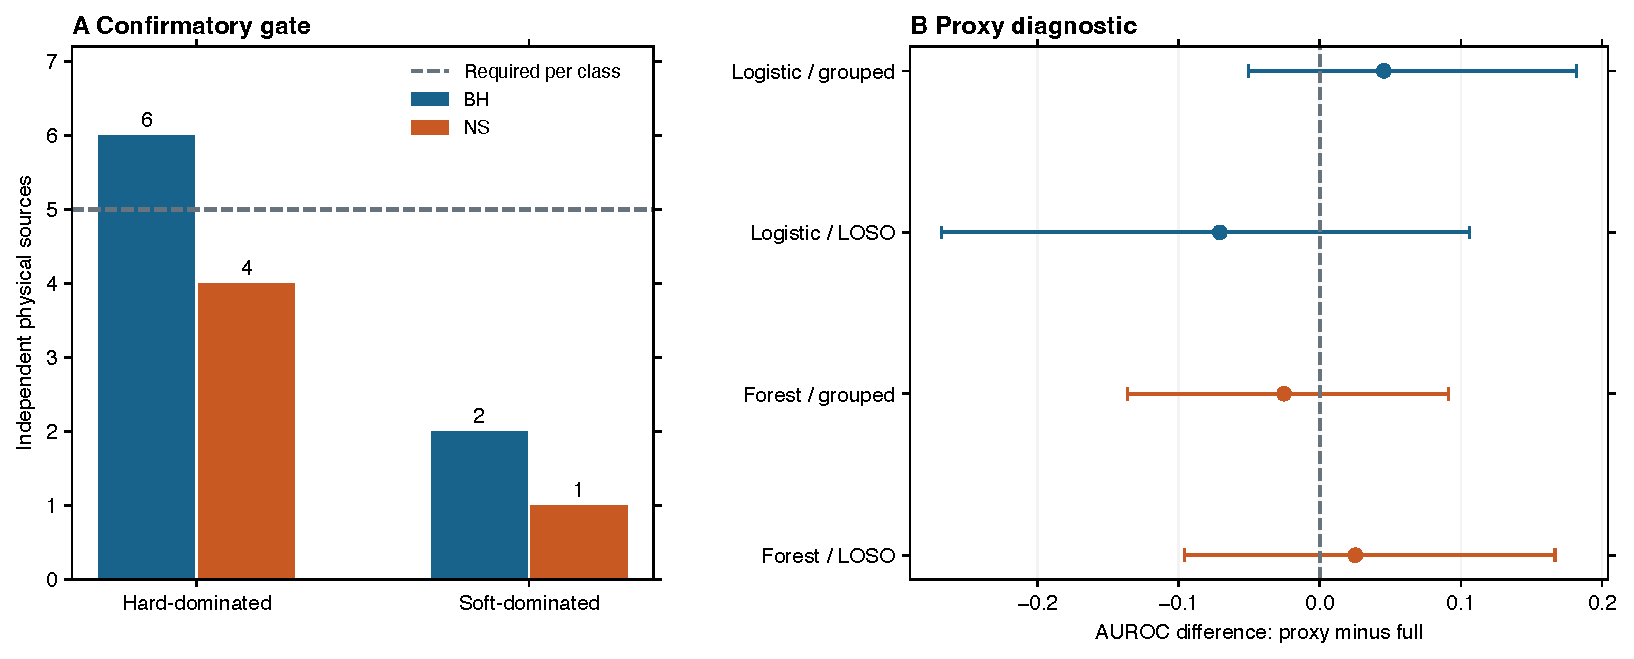
\includegraphics[width=\textwidth]{figures/figure_6_state.pdf}
\caption{Spectral-state controls and feasibility. Left: numbers of independent BH and NS systems supported in the proposed hard- and soft-dominated common regimes, compared with the pre-specified requirement of five systems per class. Right: paired proxy-minus-full-spectrum AUROC differences with conditional source-bootstrap intervals in the frozen expanded cohort. Intervals crossing zero do not establish equivalence between the representations. The hardness--intensity diagnostic does not substitute for physical state matching, and no state-matched classifier result is shown because the feasibility criterion was not met.}
\label{fig:6}
\par\smallskip
\begin{minipage}{\textwidth}
\footnotesize
\textbf{Alt text:} The left panel compares the available numbers of independent BH and NS systems in hard- and soft-dominated common regimes with a five-per-class feasibility threshold. The right panel shows paired differences in source-level AUROC between the coarse hardness--intensity representation and the full spectral representation, with conditional bootstrap intervals.
\end{minipage}
\end{figure*}

\section{Discussion}
\label{sec:discussion}

\subsection{Unseen-source generalization and source-associated structure}

Useful source-level BH/NS ranking persists when complete physical systems are withheld from training in the selected RXTE/PCA cohort. This distinction is important because source-grouped and leave-one-source-out (LOSO) evaluation prevent spectra from a held-out binary from entering the corresponding training set. The ranking signal also persists after independently executed HEASoft/CALDB processing and under the declared common instrumental-support restrictions. These controls support the conclusion that the source-disjoint result is not confined to a single archived spectral representation.

Previous X-ray-binary classification studies have already established important precedents for source-wise and leave-one-source-out evaluation \citep{Gopalan2015,Pattnaik2021,deBeurs2022}. The present result should therefore not be interpreted as establishing source exclusion itself as a new validation strategy. Rather, the contribution is the combination of source-disjoint evaluation with a source-label randomization diagnostic of whether repeated-source structure can itself support prediction.

The source-label randomization experiment provides that diagnostic. Arbitrary labels assigned at the level of the physical source remain predictable under observation-wise splitting despite removal of the true BH/NS mapping, whereas the median grouped performance returns close to chance. Repeated-source overlap can therefore expose source-associated information that supports prediction without requiring the genuine compact-object association. This provides a concrete reason not to interpret observation-wise performance automatically as evidence of transfer to a previously unseen binary.

The randomization result complements the paired comparison on the true labels, for which the observation-minus-grouped AUROC intervals include zero. It demonstrates the existence of an exploitable source-associated pathway but does not quantify what fraction of the real-label observation-wise performance arises from that pathway. Likewise, the source-identification diagnostic supports the presence of information associated with physical identity but does not identify its origin. The term ``source fingerprint'' is therefore descriptive rather than mechanistic: literal memorization is not established.

\subsection{What information supports the classification?}

The present experiments do not uniquely determine which physical or instrumental properties support BH/NS discrimination. Several non-exclusive possibilities remain, including differences in accretion-state occupancy, spectral hardness and intensity, absorption, source-specific spectral structure, detector response and observing epoch. These possibilities should be regarded as hypotheses rather than measured causal contributions.

The coarse hardness--intensity diagnostic is informative in this respect. A low-dimensional detector-space representation retains substantial class-associated ranking, showing that substantial predictive information is already present in broad spectral shape and intensity. However, the paired proxy-versus-full-spectrum comparisons do not establish equivalence, and the proxy variables are not independently justified physical-state labels. The analysis therefore does not show that coarse spectral coordinates completely mediate the full-spectrum classification.

The state-controlled investigation places an additional limit on physical interpretation. BH and NS native state taxonomies cannot be mapped to a common regime solely from observed hardness, and the pre-specified source-diversity criterion for a confirmatory matched analysis was not met. Physical spectral-state independence consequently remains unresolved. The source-disjoint ranking may reflect spectral structure associated with compact-object class, differences in state occupancy, other source-associated properties, or some combination of these effects.

Instrumental pathways are similarly constrained but not eliminated. Independently executed processing, matched-ObsID comparisons and common-support restrictions retain the ranking signal, while metadata-only models do not reproduce the spectral performance. These controls argue against the ranking being explained solely by the recorded metadata or by one processing implementation, but they cannot exclude unmeasured confounding or interactions between instrumental conditions and the spectra. The present analysis therefore does not establish that either classifier has isolated a unique physical signature of compact-object type.

\subsection{Ranking, threshold classification and scope of use}

The distinction between ranking and fixed-threshold classification is important for interpreting the reported performance. AUROC measures how well source scores order BH and NS systems across the cohort, whereas balanced accuracy is the mean of the class-specific recalls after application of a specified decision threshold. A transformation or systematic shift of the scores can preserve much of their ordering while moving several sources to the same side of the threshold. High AUROC and more modest balanced accuracy are therefore not contradictory outcomes.

This distinction is particularly visible in the LOSO results, where high source-level AUROC is accompanied by more modest balanced accuracy at the fixed 0.5 threshold. The threshold was not optimized against the outer-test predictions, and calibration suitable for deployment has not been demonstrated. Mean-log-odds pooling provides a reproducible source-level summary of repeated observations, but the resulting score should not be interpreted automatically as a calibrated posterior probability.

The classifiers should therefore be interpreted primarily as ranking tools within the selected cohort rather than as deployment-ready systems for secure compact-object identification. Applications requiring decisions for individual newly observed binaries would require separately justified score calibration, operating thresholds and validation in a population that matches the intended use. Machine-learning predictions also do not replace dynamical measurements, thermonuclear bursts, pulsations or other physical evidence used to establish secure compact-object classifications.

\subsection{Astrophysical and methodological implications}

The persistence of source-disjoint ranking shows that detector-space RXTE/PCA spectra contain BH/NS-associated information that transfers across at least some held-out physical systems in the selected cohort. This remains scientifically informative even without unfolding every observation into a specific emission model. The result is nevertheless conditional on the represented systems, their observing histories and the evidence used to define their labels. In particular, the infeasible state-matched experiment means that the transferable information cannot yet be separated cleanly from differences in physical-state occupancy.

The analysis also has broader implications for machine-learning studies in which many measurements are obtained from comparatively few astronomical objects. The appropriate evaluation unit depends on the intended inference. Observation-wise evaluation can be suitable when the goal is prediction of additional measurements from partly familiar systems. Claims about transfer to previously unseen physical objects, however, require evaluation in which those objects are excluded from training. Reporting these settings separately makes the intended generalization target explicit.

Physical identity must also be resolved before the split is constructed. Aliases that place observations from one astronomical system into different groups can defeat nominal source separation even when catalogue strings are handled consistently in code. Source-aware weighting, source-level uncertainty and source-label randomization then address distinct problems: weighting limits domination by heavily observed systems, source-bootstrap resampling aligns uncertainty with the declared inference unit, and randomization tests the predictive consequences of repeated physical identity. None substitutes for the others.

Taken together, the results support useful source-disjoint BH/NS ranking within the selected RXTE/PCA cohort while placing explicit limits on its physical and operational interpretation. The appropriate conclusion is not a universal compact-object classifier, but evidence that class-associated spectral information persists across held-out physical systems and that repeated-source structure must be treated explicitly when evaluating astronomical machine-learning systems.

\section{Limitations}
\label{sec:11}

The analysed RXTE/PCA cohort is selected rather than population-complete. Secure-label requirements, deterministic observation sampling, successful product acquisition and subsequent quality cuts restrict the systems and observations represented. The number of independent physical systems is also substantially smaller than the number of spectra, with particularly limited BH representation and unequal BH/NS source counts. These features constrain the precision of source-level generalization estimates and the stability of fixed-threshold classification. State coverage is likewise non-random because archival availability and the availability of published state evidence can jointly determine which observations enter the analysis.

The measurements are specific to RXTE/PCA and remain in detector space. The primary and independently processed representations differ in detector selection, screening, background estimation, response construction and exposure handling. Although matched-ObsID and common-support analyses reduce some of these differences, residual detector- and epoch-associated confounding may remain. The propagated spectral statistical uncertainties also do not encompass all calibration and background-model systematics. No independent-mission validation or quantitative estimate of transfer to another X-ray instrument is provided.

Physical spectral-state dependence remains unresolved. The available literature-supported catalogue did not satisfy the pre-specified source-diversity criterion required for the confirmatory state-matched experiment, and the classifier was therefore not evaluated under matched physical-state conditions. The coarse hardness--intensity diagnostic does not substitute for that experiment. Consequently, the source-disjoint classification result remains conditional on the state mixture represented in the selected cohort, and stronger physical interpretation would require additional independently supported systems.

The reported source scores are not established as calibrated posterior probabilities, and classification at the fixed threshold is less stable than source ranking. Conditional source-bootstrap intervals resample the completed source-level predictions but do not repeat preprocessing, hyperparameter selection or model fitting, and therefore do not represent full training or cohort-composition uncertainty. The small number of independent systems also limits the resolution of the inner model-selection procedure. Finally, the stage-frozen local protocols provide an audit trail for individual analyses but do not constitute external preregistration of the complete study. Sensitivity analyses are correlated robustness checks rather than independent discoveries and are not combined into a formal multiple-testing significance claim.

\section{Conclusions}
\label{sec:13}

Strong source-level BH/NS ranking remains after complete physical-source holdout in the selected RXTE/PCA cohort and persists after independently executed HEASoft/CALDB processing, matched-observation comparisons and restrictions to common instrumental support. The result therefore concerns discrimination across held-out systems represented by this cohort rather than universal compact-object identification.

Source-level label randomization provides a complementary warning about repeated-source evaluation. Arbitrary labels attached to physical systems remain strongly predictable when observations of the same systems can occur in both training and testing, but median performance returns close to chance under source-grouped evaluation. This provides direct evidence for exploitable source-associated structure and shows that prediction of another observation from a partly familiar binary is a different inference problem from transfer to a previously unseen physical system.

The physical origin of the transferable signal remains unresolved. Coarse hardness--intensity information carries substantial class-associated information, but physical spectral-state independence was not established because the pre-specified source-diversity requirement for the confirmatory state-matched experiment was not met. Score calibration, prospective deployment and transfer to other X-ray missions also remain unestablished. When the intended inference concerns previously unseen astronomical objects, evaluation should preserve physical-source separation and state the corresponding limits of interpretation explicitly.

%\section*{Acknowledgements}

%\AuthorTODO{acknowledgements and funding, including grant identifiers or an author-confirmed absence of specific funding.}

%\AuthorTODO{approve an accurate AI/computational/editorial assistance disclosure here and in the covering letter. Describe the tools, scope of use and human verification; do not certify unreviewed wording.}

%\section*{Conflict of interest}\AuthorTODO{author-approved conflict-of-interest declaration.}

%\section*{Author contributions}\AuthorTODO{author-approved contribution statement and ORCID identifiers.}

%\section*{Data availability}

%Raw RXTE archive products and mission reduction documentation are public through NASA HEASARC \citep{NASAStandard}. The retained project contains the source census, aliases and evidence, acquisition manifests, reconstructed arrays, covariance records, hashes, frozen configurations, out-of-fold predictions and fit audits. Supplement S1--S6 indexes these materials and distinguishes raw-data provenance from derived model inputs.

%TODO: deposit the author-approved code and derived-data release, select its licence, provide persistent accession identifiers, and replace this sentence with verified archive/repository links. No repository DOI or public code release is claimed here. The proposed release includes machine-readable tables and source-level predictions; publication PDFs retained for evidence review are referenced, not presumed redistributable. Detailed availability and release checks accompany the manuscript.

%\section*{Software availability}

%Scientific processing uses NumPy for numerical arrays \citep{Harris2020} and Astropy for FITS products and time handling \citep{Astropy2022}.

%Analysis code exists and has been checked locally, as described in Section~\ref{sec:12}. \AuthorTODO{provide the approved public code release, version, licence and persistent identifier. A public release and clean-host raw-data reproduction have not yet been established.}

\balance\bibliographystyle{mnras}\bibliography{references}
\label{lastpage}
\end{document}
